% !TeX spellcheck = pl_PL
\documentclass[8pt,a3paper]{article}
\usepackage{polski}
\usepackage[utf8]{inputenc}
\usepackage{amsmath}
\usepackage{amsfonts}
\usepackage{enumitem}
\usepackage{amssymb}
\usepackage{graphicx}
\usepackage{multirow}
\usepackage{hhline}
\usepackage{listings}
\usepackage{siunitx}
\usepackage{hyperref}
\usepackage{color}
\usepackage[dvipsnames]{xcolor}
\usepackage{scrextend}
\usepackage{enumitem}
\usepackage{listings}
\usepackage{float}
\usepackage{placeins}
\usepackage[makeroom]{cancel}
\usepackage[left=0.50cm,right=0.50cm,top=0.7cm,bottom=0.70cm,columnsep=14pt]{geometry}
\setlength{\columnseprule}{0.2pt}
\usepackage{microtype} % Slightly tweak font spacing for aesthetics
\usepackage{enumitem} % Customized lists
\usepackage{multicol}


\newenvironment{rcases}
    {\left.\begin{aligned}}
    {\end{aligned}\right\rbrace}

\usepackage{pgf}
\usepackage{tikz}
\usetikzlibrary{positioning,arrows,automata}
\usetikzlibrary[automata,calc]
\usepackage{verbatim}
\tikzstyle{every state}=[fill=white,draw=black,text=black,minimum size=10pt]
\tikzstyle{every node} = [fill=white,text=black,scale=0.9]

\begin{document}
\begin{multicols*}{3}
	Niech $f(n)$ oraz $g(n)$ będą funkcjami ze zbioru $\mathbb{N}$ w zbior $\mathbb{R}$. Powiemy, że $f=O(g)$ (co oznacza "$f$ rośnie nie szybciej niż $g$"), jeśli istnieje stała $c>0$ taka, że $f(n)\leq cg(n)$\\
	$1,\log\log n,\log n, (\log n)^{c},n^{c} c<1, n,n\log n,n^{2},n^{c},c^{n},$\\
	$log_{a}b=c \Leftrightarrow a^{c}=b \quad log_{a}a = 1 \quad log_{e}a*b = log_{e}a + log_{e}b \\ log_{b}a^{n} = nlog_{b}a \quad log_{b}a= \frac{log_{c}a}{log_{c}b} \qquad log_{b}(\frac{1}{a})= - log_{b}a \\log_{b}a=\frac{1}{log_{a}b}\qquad a^{log_{b}n} = n^{log_{b}a} \quad log_{a}\frac{x}{y}=log_{a}x-log_{a}y $\\
	$ n! = o(n^{n}), \omega(2^{n}) \quad \log(n!) = \Theta(n\lg n)$ \\
	$ \sum_{j=i}^{n} j = \frac{n(n+1)}{2} - \frac{i(i-1)}{2} \quad 
	\sum_{i=0}^{n} i^{2} = \frac{n(n+1)(2n+1)}{6} \\
	\sum_{i=k_{0}}^{k_{1}}\sum_{j=l_{0}}^{l_{1}}a_{i}b_{j} = (\sum_{i=k_{0}}^{k_{1}} a_{i})(\sum_{j=l_{0}}^{l_{1}} b_{j}) \\ 
	\sum_{k=1}^{n}(ca_{k}+b_{k}) = c\sum_{k=1}^{n}a_{k} + \sum_{k=1}^{n}b_{k} \\
	\sum_{k=1}^{n}k = \frac{1}{2}n(n+1) \quad \sum_{i=1}^{n}i = \frac{n(n+1)}{2}\\
	\sum_{k=0}^{n}x^{k} = \frac{1-x^{n+1}}{1-x} \quad \sum_{i=1}^{n}\frac{1}{i} = \Theta(\log n) \\
	\sum_{j=i}^{n}1=n-i \quad \sum_{i=1}^{n}1=n^{2}  \\ 
	\sum_{i=0}^{n}\log \frac{n}{i}=\sum_{i=0}^{n}\log n - \sum_{i=0}^{n}\log i$\\
	$T(n) = 2T(\lfloor n/2 \rfloor) + n \to \Theta(n\lg n) \\
	T(n) = T(\lceil n/2 \rceil) + 1 \to O(\lg n) \quad {\color{BrickRed}{\sum_{i=0}^{lgn}1}}\\
	T(n) = T(\lceil n/2 \rceil) + n \to O(n) \quad {\color{BrickRed}{\sum_{i=0}^{lgn}\frac{n}{2^{k}}}}\\
	T(n) = 2T(n/2)+n^{2} \to \Theta(n^{2}) \\ 
	T(n) = T(n/2)+T(2n/3)+n \to O(n\lg n) \\
	T(n) = 9T(n/3)+n \to \Theta(n^{2}) 
	T(n) = T(2n/3) +1 \to \Theta(\lg n) \\ 
	T(n) = 3T(n/4) + nlgn \to \Theta(n\lg n) \\
	T(n) = T(n-1)+n \to \Theta(n^{2}), T(n) = T(n-1)+1 \to \Theta(n)\\
	T(n) = 3T(n/2) + n \to O(n^{\lg 3}){\color{BrickRed}{\sum_{i=0}^{lgn}\frac{n}{2^{k}}3^{k}}}$ \\
	\textbf{ROZWIĄZYWANIE REKURENCJI}\\
	1* Metoda podstawiania \\
	 $T(n) = 4T(\frac{n}{2}+n),\qquad T(1)=\Theta(1) \\$
	 $ \bullet T(n) = O(n^{3}) \gets$ zgadujemy \\
	 Zał. ind.:$\bigvee_{k<n} T(k) \leq ck^{3}$\\
	 Krok: $ T(n)=4T(\frac{n}{2})+n \leq  4c(\frac{n}{2})^{3} +n = c\frac{n^{3}}{2}+n = cn^{3}+(n-c\frac{n^{3}}{2}) \leq cn^{3} $\\ \qquad Kiedy $n-c\frac{n^{3}}{2} \leq 0$? $\to c>2, n>2 \to$ Istnieją wartości dla których krok indukcyjny jest prawdą. Aczkolwiek ten przykład lepiej zrobić tak: zał.ind.:$\bigvee_{k<n} T(k) \leq c_{1}k^{2}-c_{2}k$ \\
	2* Drzewo rekursji \\
	$T(n)=T(\frac{n}{2})+T(\frac{n}{4})+n^{2}$
	\vspace{-0.5cm}
	 \begin{figure}[H]
		 	\centering
		 	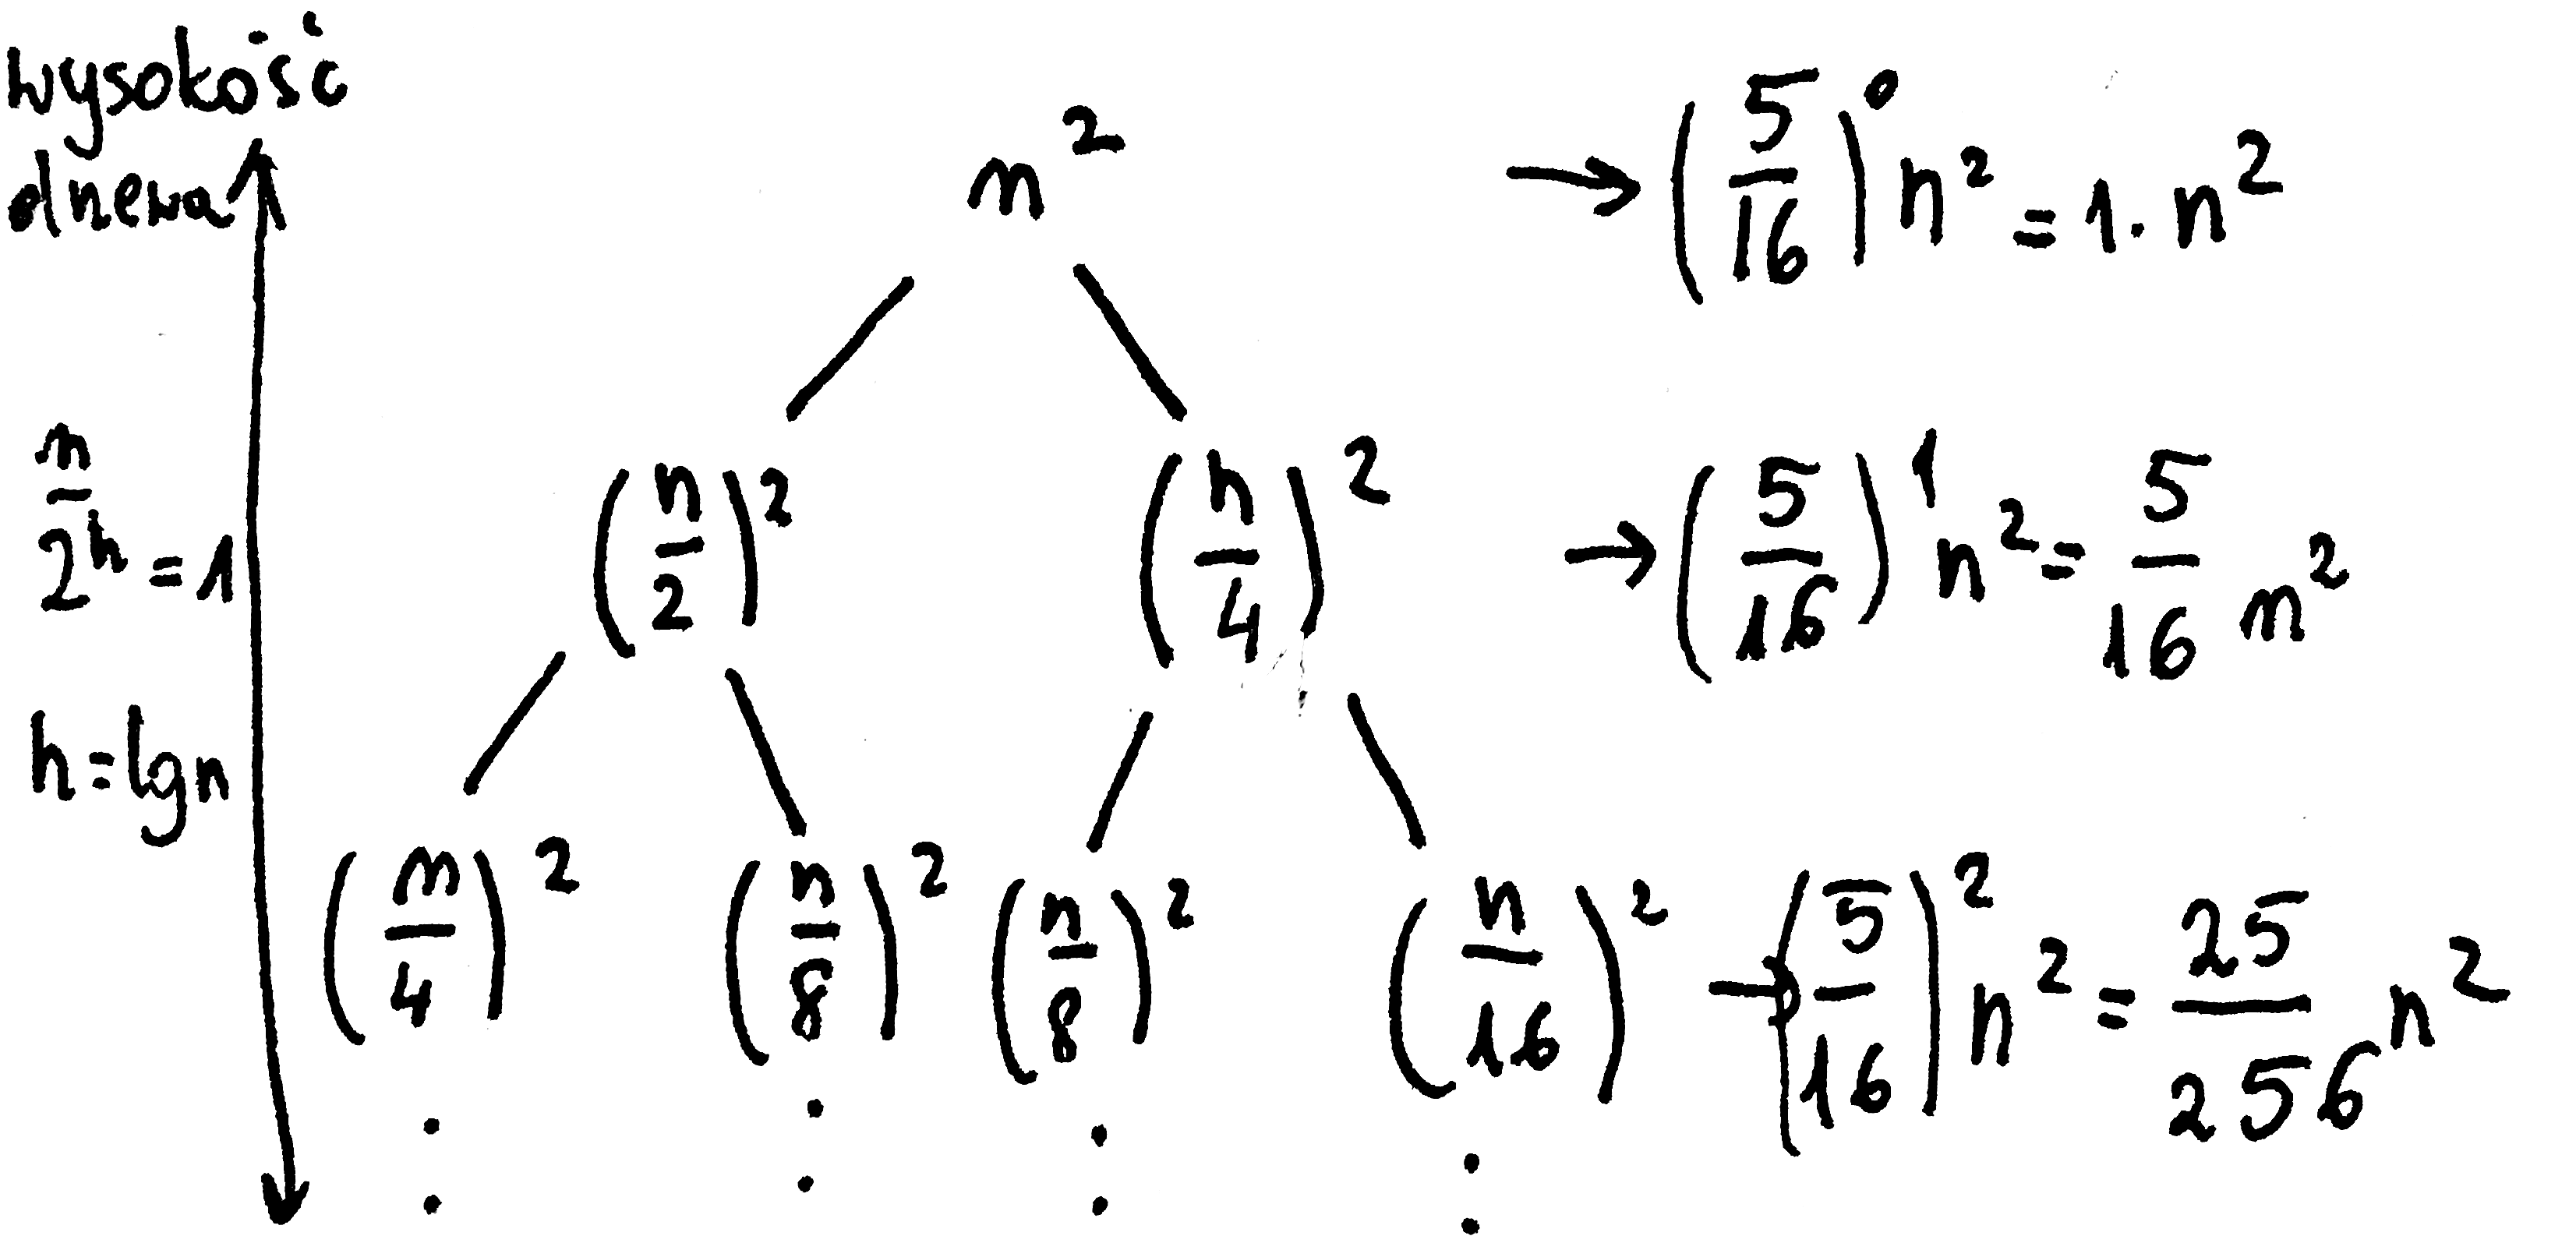
\includegraphics[width=7cm]{recursiveTree.PNG}
	 \end{figure}
	 \vspace{-0.5cm}
	liczba operacji $\to$ suma operacji w każdym wierszu \\
	$\sum_{k=0}^{\lg n} (\frac{5}{16})^{k}n^{2} \to n^{2}*\frac{16}{11}-\frac{5}{11}n^{0.4}$\\
	3* Przez zamianę zmiennych \\
	$T(n) = 2T(\sqrt{n})+\lg n$ \\
	Założenie: $n=2^{m}; \qquad T(2^{m}) = 2T(2^{\frac{m}{2}})$\\
	{\color{PineGreen}$S(m) = T(2^{m})$ \textit{drzewo}}$ \quad S(m)=2S(\frac{m}{2})+m \quad S(m)=m\lg m$ \\
	$T(n)=T(2^{m})=S(m)=m\lg m = (\lg n)(\lg\lg n)$ \\
	$n = 2^{m}, m = \lg n$ \\
	\vspace{-0.8cm}
	 \begin{figure}[H]
		 	\centering
		 	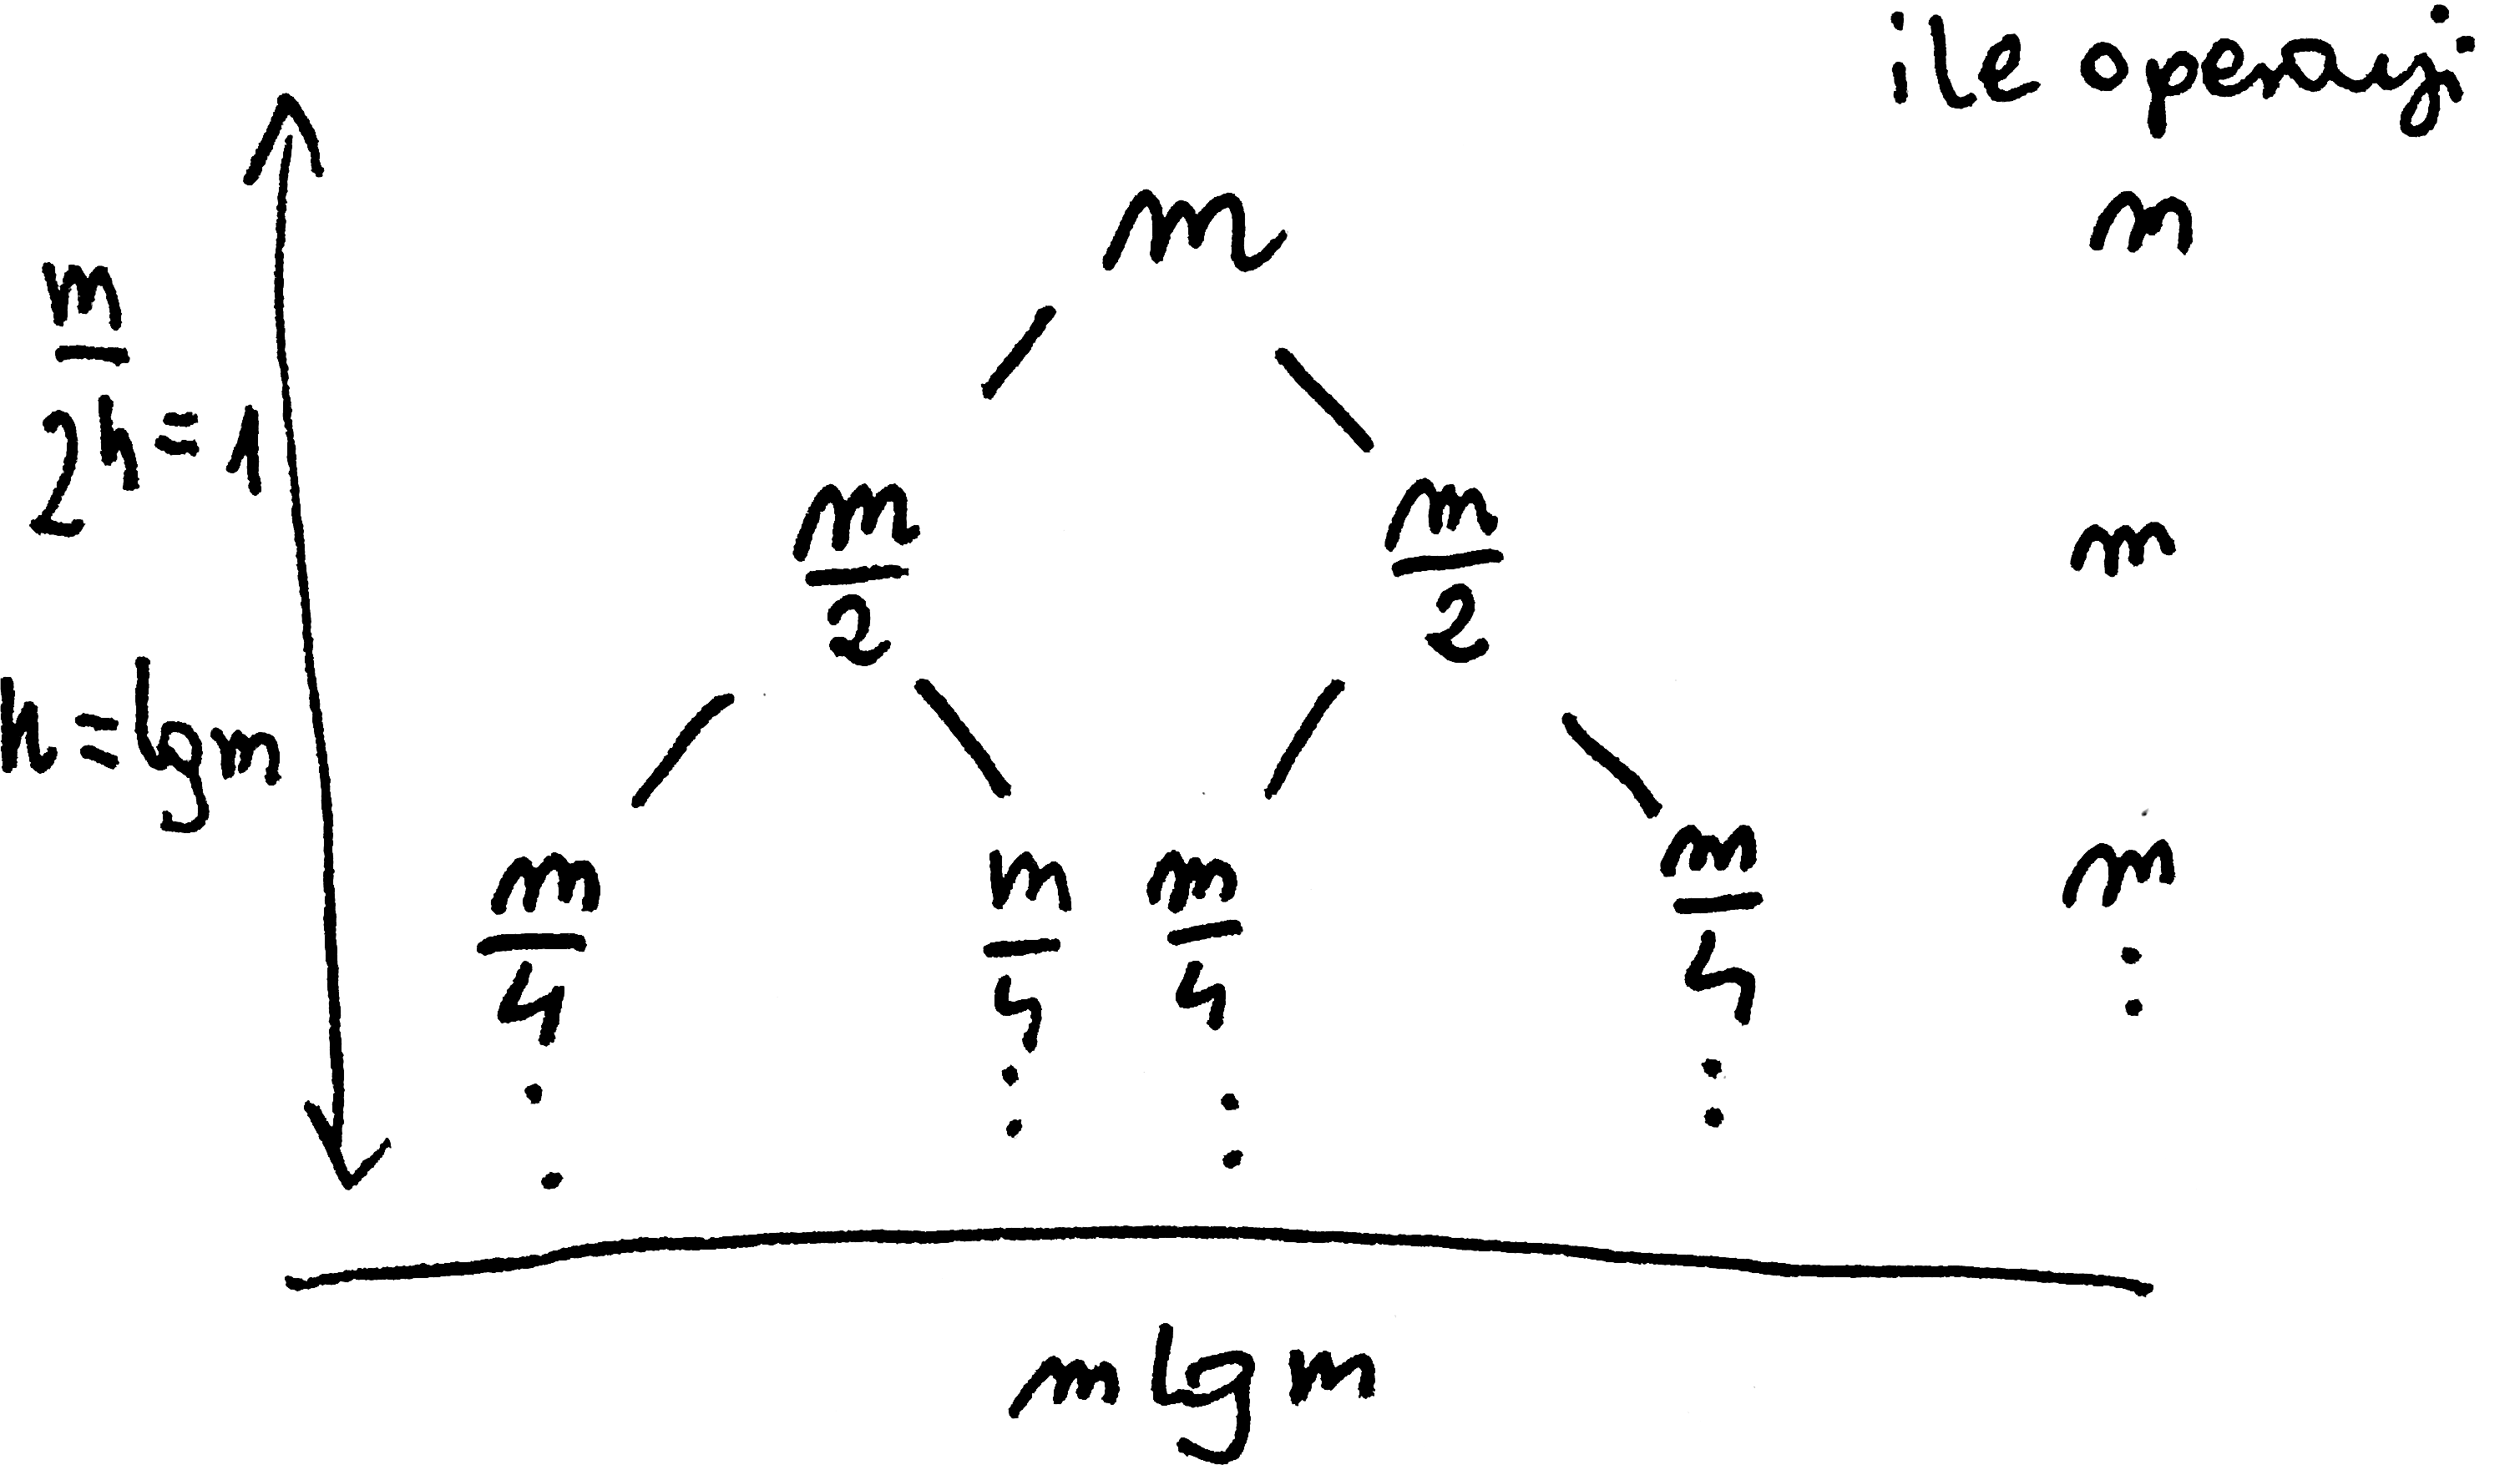
\includegraphics[width=6cm]{variableTree.PNG}
	 \end{figure} 
	 \vspace{-0.7cm}
	4* Metoda iteracyjna \\
	 $T(1)=\Theta(1); \qquad T(n) = 3T(\frac{n}{4})+n = 3(3T(\frac{n}{16})+\frac{n}{4}) = n+\frac{3}{4}n+3^{2}T(\frac{n}{16}) = n+\frac{3}{4}n + 3^{2}(3T(\frac{n}{64})+\frac{n}{16})=n+\frac{3}{4}n+(\frac{3}{4})^{2}n+3^{3}T(\frac{n}{64})= n+\frac{3}{4}n+(\frac{3}{4})^{2}n+...+(3)^{\log_{4}n}*\Theta(1)= \qquad n\sum_{k\leq0}(\frac{3}{4})^{k}=\Theta(n)$ \\
	\textbf{MASTER THEOREM}\\
	$T(n) = aT(\frac{n}{b})+O(n^{d}), \quad a>0, b>1, d \geq 0$ \\
	\[ T(n) =
	\begin{cases}
	O(n^{d})    & \quad \text{if } d>\log_{b}a\\
	O(n^{d}\log n)  & \quad \text{if } d=\log_{b}a\\
	O(n^{\log_{b}a}) & \quad \text{if } d<\log_{b}a
	\end{cases}
	\]
	\textbf{INSERTION SORT}($a,n$) \\
	for $j=2$ to $n$:\\
	.\quad key = $a_{j}$, $i = j-1$ \\
	.\quad while $i>0$ and $a_{i} > key$:\\
	.\quad.\quad $a_{i+1} = a_{i}$ , $i--$ \\
	.\quad $a_{i+1} = $ key \\
	$T(n) = \sum_{j=2}^{n}\Theta(j) = \Theta(\sum_{j=2}^{n}j) = \Theta(n^{2})$ \\
	\textbf{MERGE SORT}($A[1...n],n$) \\
	if $n==1$: return $A[1]$\\
	else: $B=A[1,...,\lfloor\frac{n}{2}\rfloor] $\\
	.\qquad $C=A[\lfloor\frac{n}{2}\rfloor-1,...,n]$ {\color{BrickRed}$B,C \to \Theta(n)$}\\
	.\qquad MergeSort($B,\frac{n}{2}$) {\color{BrickRed}$\to T(\frac{n}{2})$}\\
	.\qquad MergeSort($C, \frac{n}{2}$) {\color{BrickRed}$\to T(\frac{n}{2})$}\\
	.\qquad $A$ = Merge($B,C$) {\color{BrickRed}$\to \Theta(n)$}\\
	$T(n)=2T(\frac{n}{2})+\Theta(n)$ \\
	\vspace{-0.7cm}
	\begin{figure}[H]
	 	\centering
	 	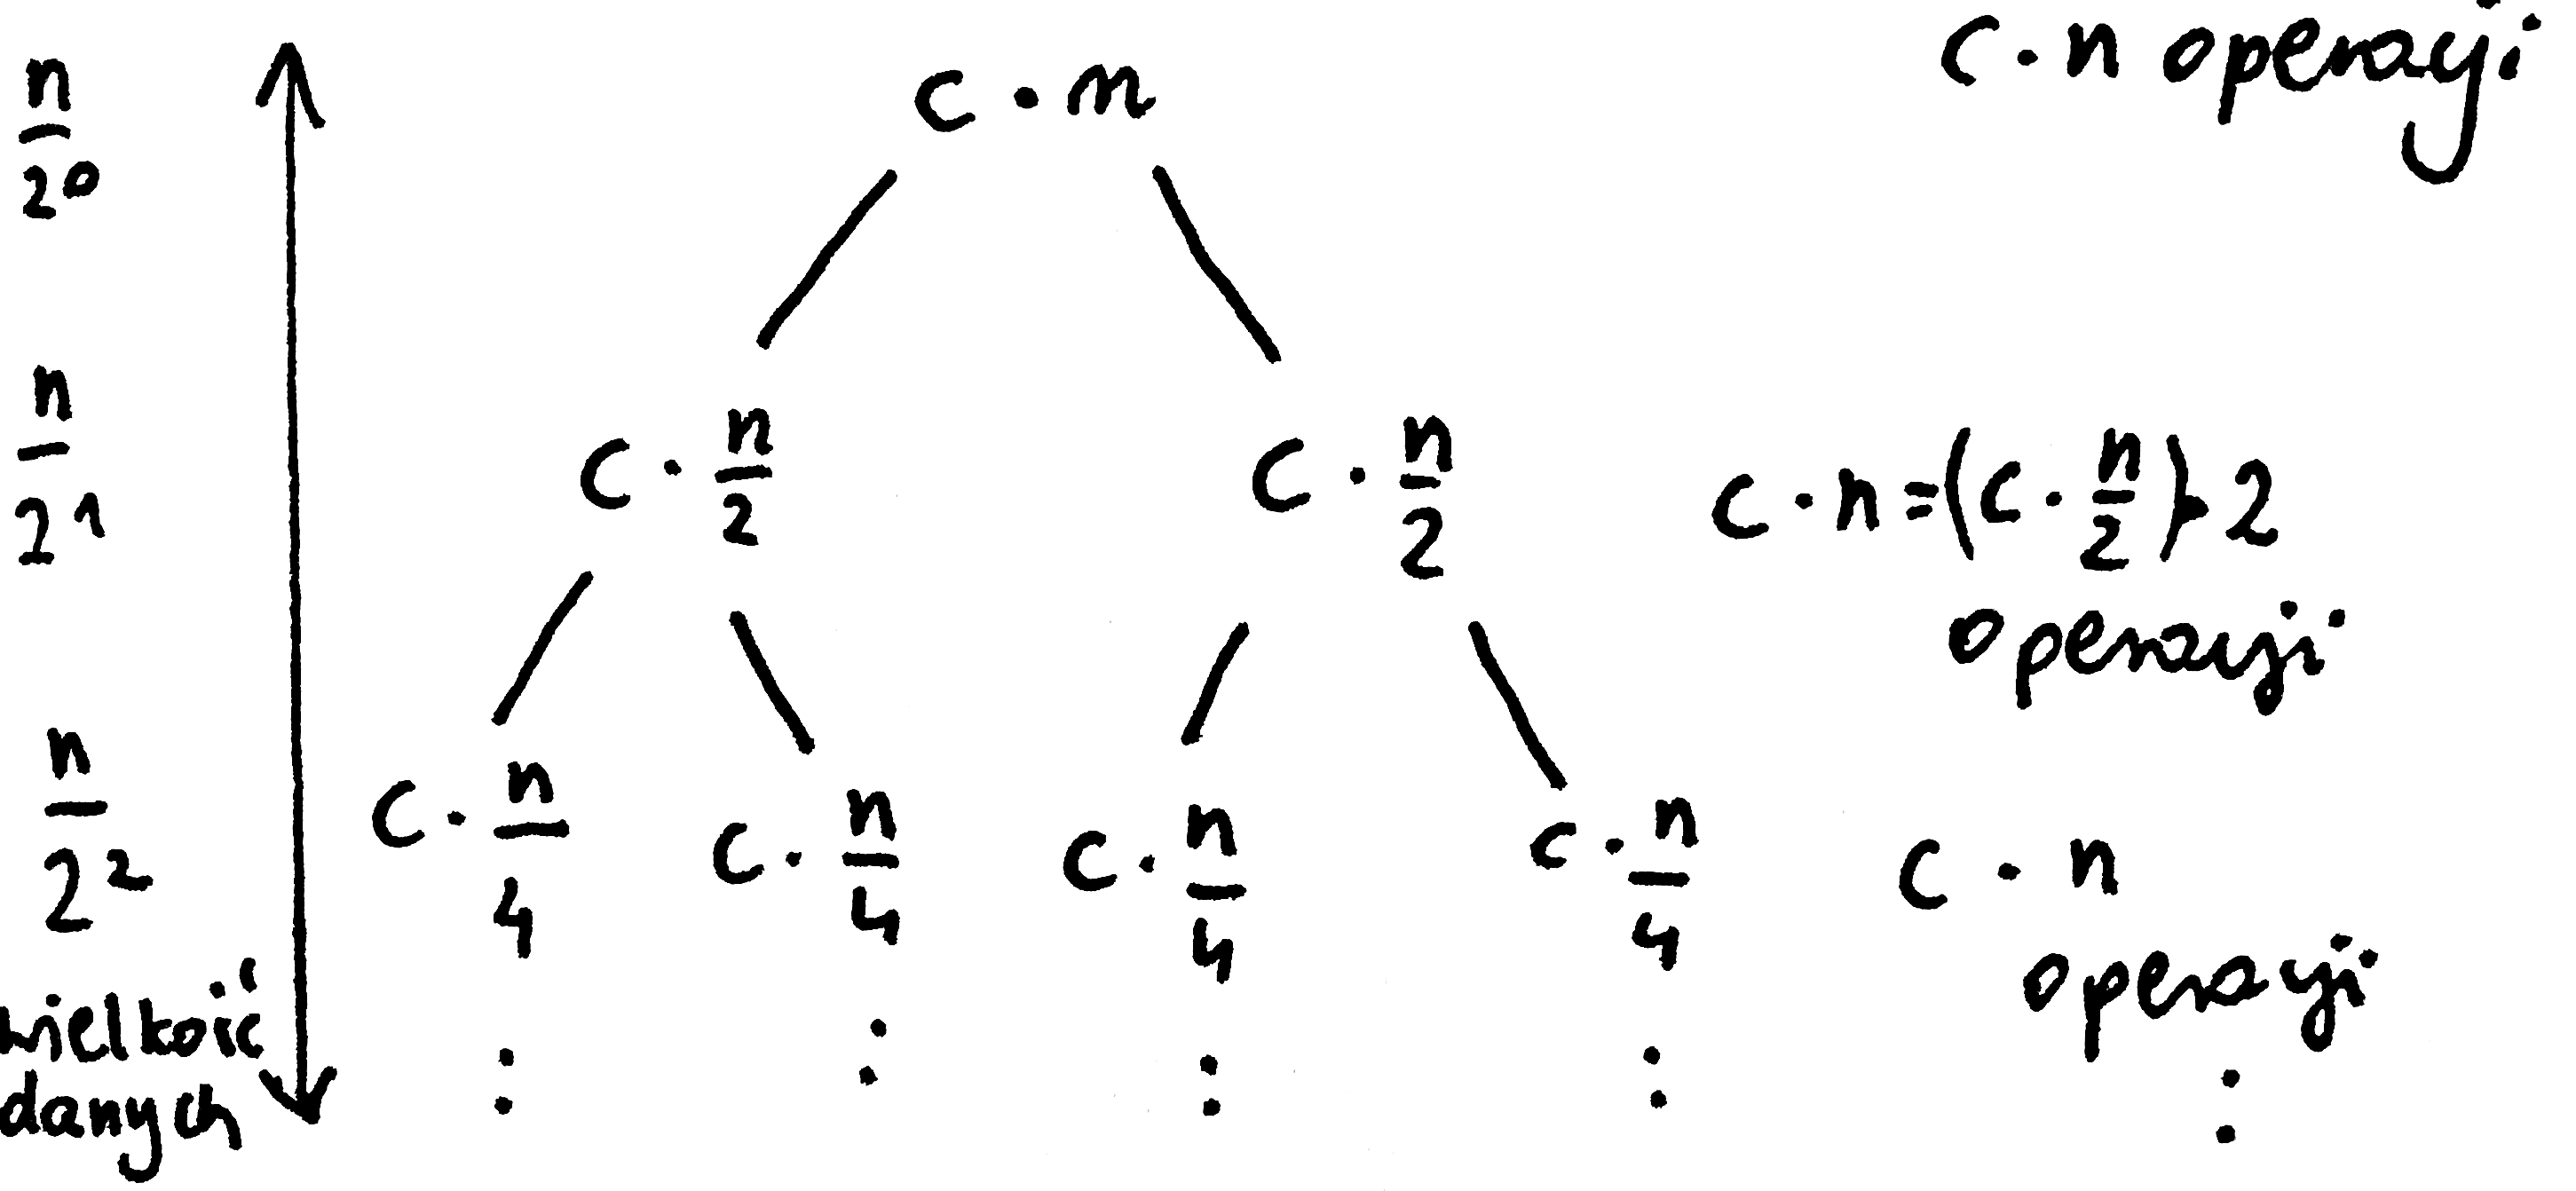
\includegraphics[width=7cm]{mergeTree.PNG}
	\end{figure}
	\vspace{-0.7cm}
	Ile mamy poziomów w tym drzewie? (wysokość drzewa)\\
	poziom $k+1$: \quad $\frac{n}{2^{k}}=1 \quad \to k=\log_{2}n$\\
	$T(n)=(c*n)*\lg n = \Theta(n \lg n)$ \\
	\textbf{DIVIDE $\&$ CONQUER} $T(n) = aT(\frac{n}{b}+O(n^{d}))$ \\ $ a \to$ liczba podproblemów, których jest $\frac{n}{b}$, $O(n^{d}))\to$ scalanie podproblemów \\
	\textbf{BINARY SEARCH}($x, A, p, q$) \\
	input: posortowana tablica $A$, output: znaleźć element $x$
	$y = a_{\lfloor \frac{p+q}{2} \rfloor} $ \\
	if $y==x$ : return $\lfloor \frac{p+q}{2}\rfloor $\\
	else if $y<x$:
	\quad BinarySearch($x,A,\lceil \frac{p+q}{2}\rceil ,q)$ \\
	else:
	\quad BinarySearch($x,A,p, \lfloor \frac{p+q}{2}\rfloor -1$)\\
	$T(n)=T(\frac{n}{2})+O(1) \to O(\log n)$ \\
	\textbf{QUICK SORT}($A,p,q$) \\
	if $p<q$ : \\
	.\quad $pivot$ = Partition($A,p,q$) \\
	.\quad QuickSort($A,p,pivot-1$) \\
	.\quad QuickSort($A,pivot+1,q)$\\
	Best Case $\to$ każdy Partition będzie zwracał pivota na środku $\to \Theta(n\log n)$ \\
	Worst Case $\to$ pivot albo najmniejszym albo największym elementem tablicy (zwraca niezmienioną tablicę) $\to T(n)=T(n-1)+\Theta(n) \to \Theta(n^{2})$ \\
	Average Case $\to \Theta(n \log n)$ \\
	PARTITION($A,p,q$) $\to \Theta(n)$\\
	$x$ = SelectPivot($A,p,q$) \\
	$pivotValue$ = $A[x]$ \\
	swap($x, q$) \\
	$index = p$
	for $j=p$ to $q-1$: \\
	.\quad if $A[j] \leq pivotValue$: \quad swap($j,index), index++$ \\
	swap($index,q)$\\
	return $index$ \\
	\textbf{COUNTING SORT}($A,n,k$) $\gets$ sortowanie liniowe\\
	for $i=1$ to $k$: {\color{BrickRed}$\to \Theta(k)$ }\\
	.\quad $C[i]=0$ \\
	for $j=1$ to $n$: {\color{BrickRed}$\to \Theta(n)$} \\
	.\quad $C[A[j]]++$ \\
	for $i=2$ to $k$:  {\color{BrickRed}$\to \Theta(k)$} \\
	.\quad $C[i] = C[i] + C[i-1]$ \\
	for $j=n$ downto $1$: {\color{BrickRed}$\to \Theta(n)$} \\
	.\quad $B[C[A[j]]] = A[j]$ \\
	.\quad $C[A[j]]--$ \\
	Złożoność: $\Theta(n+k)$, jeśli $k=\Theta(n)$ to $\Theta(n+k) = \Theta(n)$ $k$ – rozpiętość danych,różnica między maksymalną a minimalną wartością.  \\
	STABLE SORTING PROPERTY $\to$ jeśli dla równych sobie elementów po posortowaniu zachowana jest kolejność (zachodzi dla Counting Sort i Radix Sort).
	\textbf{RADIX SORT}$(a,d)$ \\
	for $i=0$ to $d$: posortuj stabilnie ciągi według $i$-tej pozycji \\
	b - liczba bitów w słowie, r - liczba bitów w "cyfrze" \\
	k - ilość wartości jakie może przyjmować cyfra,rozmiar alfab.\\
	d - ilość cyfr w słowie, n - ilość danych do posortowania \\
	$\Theta(d(n+k)).$ Jeśli sortowanie jest stabilne to $\Theta(n+k)$. Jeśli $d$ jest stała, a $k=O(n)$ to sortowanie działa w czasie liniowym. \\
	$2^{b}=scope$ \\
	if $b<\lfloor \lg n \rfloor {r=b}$ \\
	else: ${r =\lfloor \lg n \rfloor} $ \\
	$k=2^{r}, d = \lceil \frac{b}{r} \rceil $\\
	Mamy $n$ liczb $b$-bitowych i dodatnią liczbę całkowitą $r \leq b$. Za pomocą RS możemy posortować te liczby w czasie $\Theta((\frac{b}{r})(n+2^{r}))$, jeśli stosowane w niej stabilne sortowanie zajmuje czas $\Theta(n+k)$ dla danych wejściowych należących do przedziału $0-k$.\\
	Sortowanie przez zliczania zastosowane z $k=2^{2}$. \\
	Minimalizacja wartości wyrażenia  $\Theta((\frac{b}{r})(n+2^{r}))$: \\
	Jeśli $b \geq \lfloor \lg n \rfloor$ to biorąc $r=\lfloor \lg n \rfloor$, dostajemy najlepszy czas. Jeśli $b < \lfloor \lg n \rfloor$, to dla dowolnego $r \leq b$ mamy $(n+2^{r}) = \Theta(n)$, biorąc $r=b$ dostajemy czas $((\frac{b}{b})(n+2^{b})) = \Theta(n)$, który jest asymptotycznie optymalny. \\
	STATYSTYKI POZYCYJNE $\to$ k-ty największy el. tablicy \\
	\textbf{RAND SELECT} ($A,p,q,i$): \\
	if $p==q$: return $A[p]$ \\
	$r =$ Rand-Partition($A,p,q$) \\ \textit{// r - index pivota po zrobieniu partition całego A} \\
	$k= r - p+1$ \textit{// k- index pivota, ale A[p..q]} \\
	if $i==k$: return $A[r]$\\
	if $i<k$: return RandSelect($A,p,r-1,i$)\\
	else: return RandSelect($A,r+1,q,i-k$)\\
	Worst Case $\to O(n^{2})$ \qquad Best Case$\to O(n)$\\
	\textbf{SELECT} ($A,n,k$): \\
	j.w. tylko inny Partition: \\
	1. podziel zbiór n elementowy na $\lceil \frac{n}{5} \rceil$ zbiorów po 5 elementów \\
	2. wyznacz medianę każdej grupy (np. Insertion Sortem) \\
	3. użyj rekurencyjnie Select(), aby wyznaczyć medianę median \\
	4. użyj mediany median jako pivota do Partition() dzielącego zbiór na $k$ w dolnej i $n-k$ elementów w górnej części \\
	5. rekurencyjnie Select() na odpowiedniej części podziału, aby wyznaczyć $i-ty$ element w dolnej lub $(i-k)$-ty w górnej części. \\
	\textbf{BINARY SEARCH TREE}\\
	INORDER TREE WALK($x$) $\to O(n)$ \\
	if $x \neq null$: \\
	.\quad ITW($x.left$) \\
	.\quad print $x$ \\
	.\quad ITW($x.right$) \\
	TREE-SEARCH($x,key$) $\to O(h),$ szukamy wartości key \\
	if $x==null$: return null \\
	if $x.value == key$: return$ x $\\
	else if $x.value > key$: \quad Tree-Search($x.left, key$) \\
	else: \quad Tree-Search($x.right, key$) \\
	INSERT($x,key$) $\to O(h$)\\
	DELETE($x,key$) $\to O(h$) \\
	MINIMUN $\to O(h)$, idziemy najbardziej w lewo\\
	MAXIMUM $\to O(h)$, idziemy najbardziej w prawo\\
	SUCCESOR($x$) $\to O(h)$ \\
	if $x.right \neq null$: return Minimum($x.right$) \\
	$p = x.parent$ \\
	while $p \neq null$ and $x==p.right$): \\
	.\quad $x=p$ \\
	.\quad $p=p.parent$ \\
	return $p$ \\
	\textbf{RED BLACK TREE} \\
	$\bullet$ każdy węzeł jest czarny albo {\color{BrickRed}czerwony} \\
	$\bullet$ korzeń i liscie są czarne \\
	$\bullet$ jeśli węzeł jest {\color{BrickRed}czerwony} to jego synowie są czarni \\
	$\bullet$ każda prosta ścieżka z korzenia do liścia ma taką samą liczbę czarnych węzłów \\
	\vspace{-0.8cm}
	 \begin{figure}[H]
		 	\centering
		 	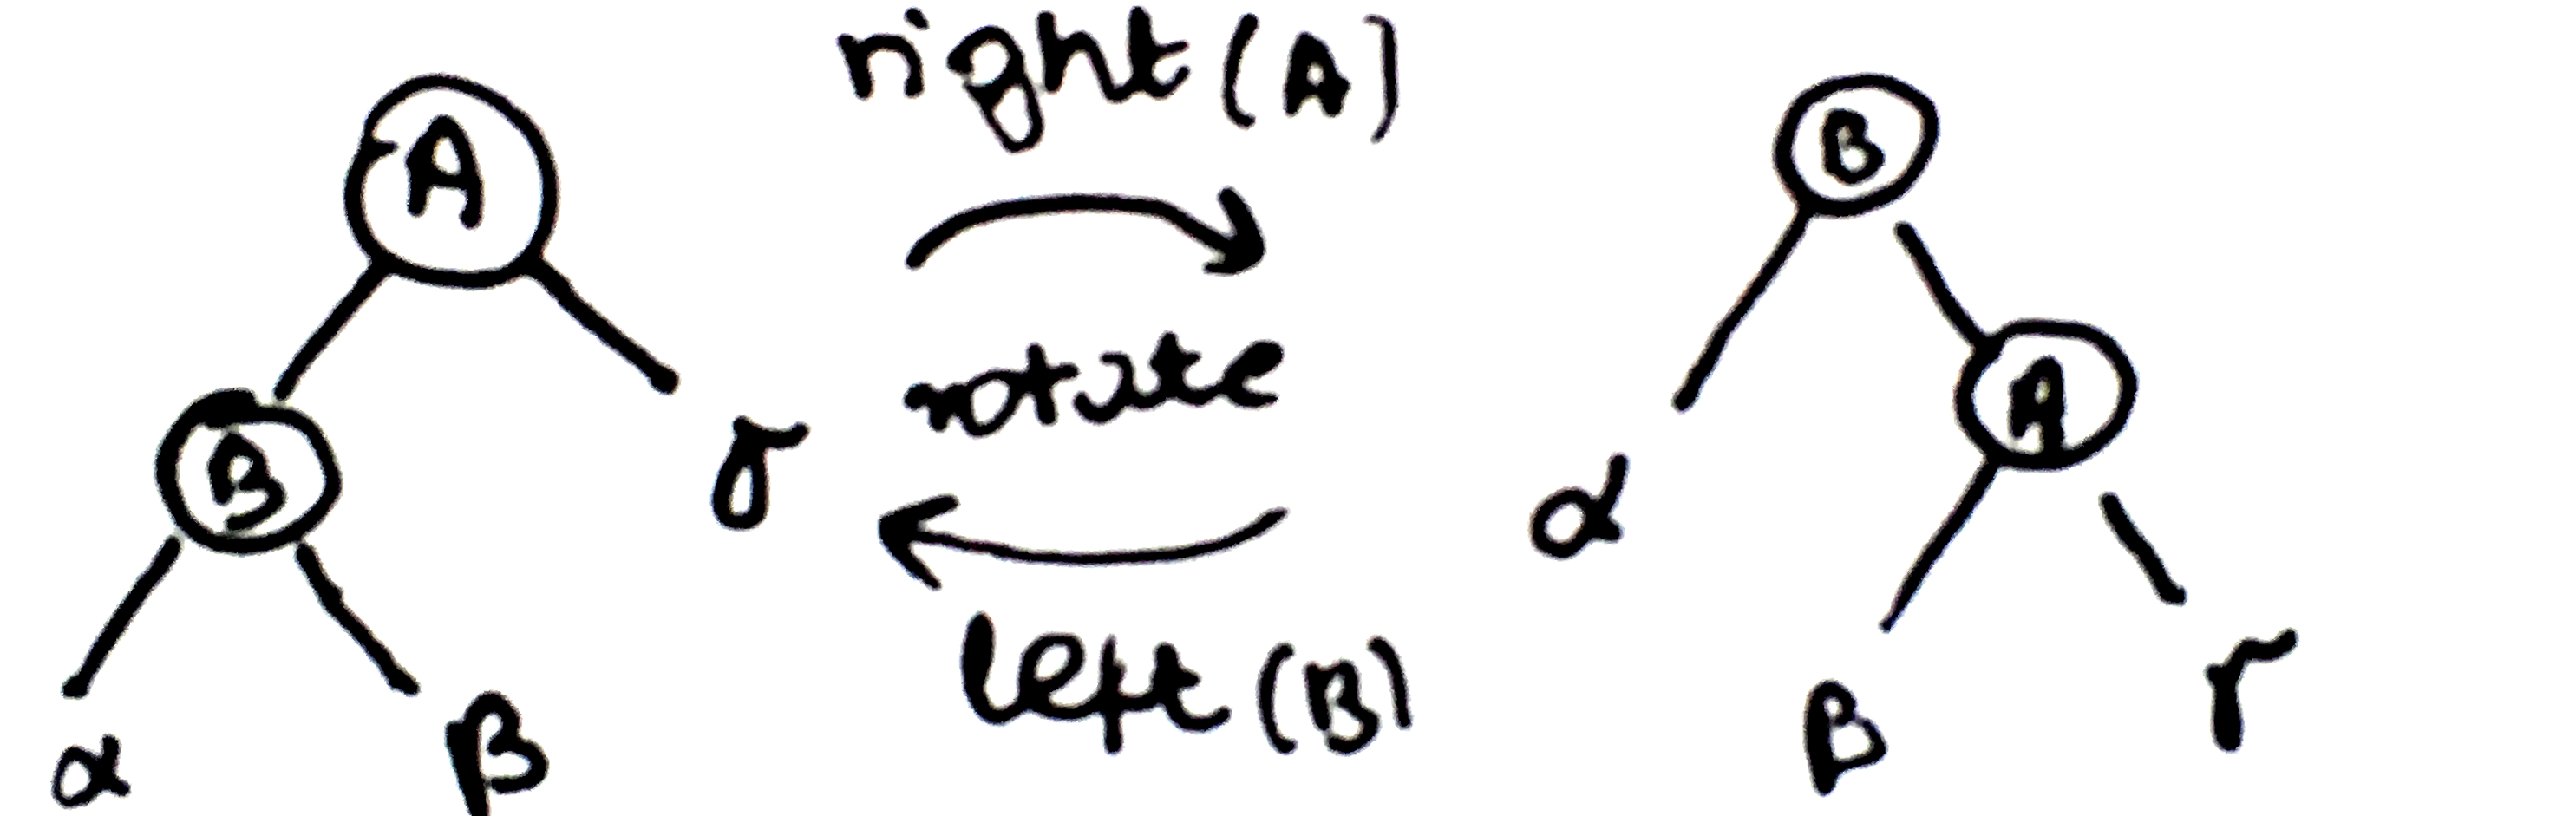
\includegraphics[width=5cm]{rotate.PNG}
	 \end{figure}
	 \vspace{-0.6cm}
	RB-INSERT($x$) $\to O(\log n)$ \\
	Wstawiamy jak w BST i naprawiamy do własności RBTree:
	\vspace{-0.5cm}
	 \begin{figure}[H]
		 	
		 	\includegraphics[width=5cm]{insert.PNG}
	 \end{figure}
	 \vspace{-0.65cm}
	RB-DETELE($x$) $\to O(\log n)$:  \\
	\vspace{-0.75cm}
	 \begin{figure}[H]
		 	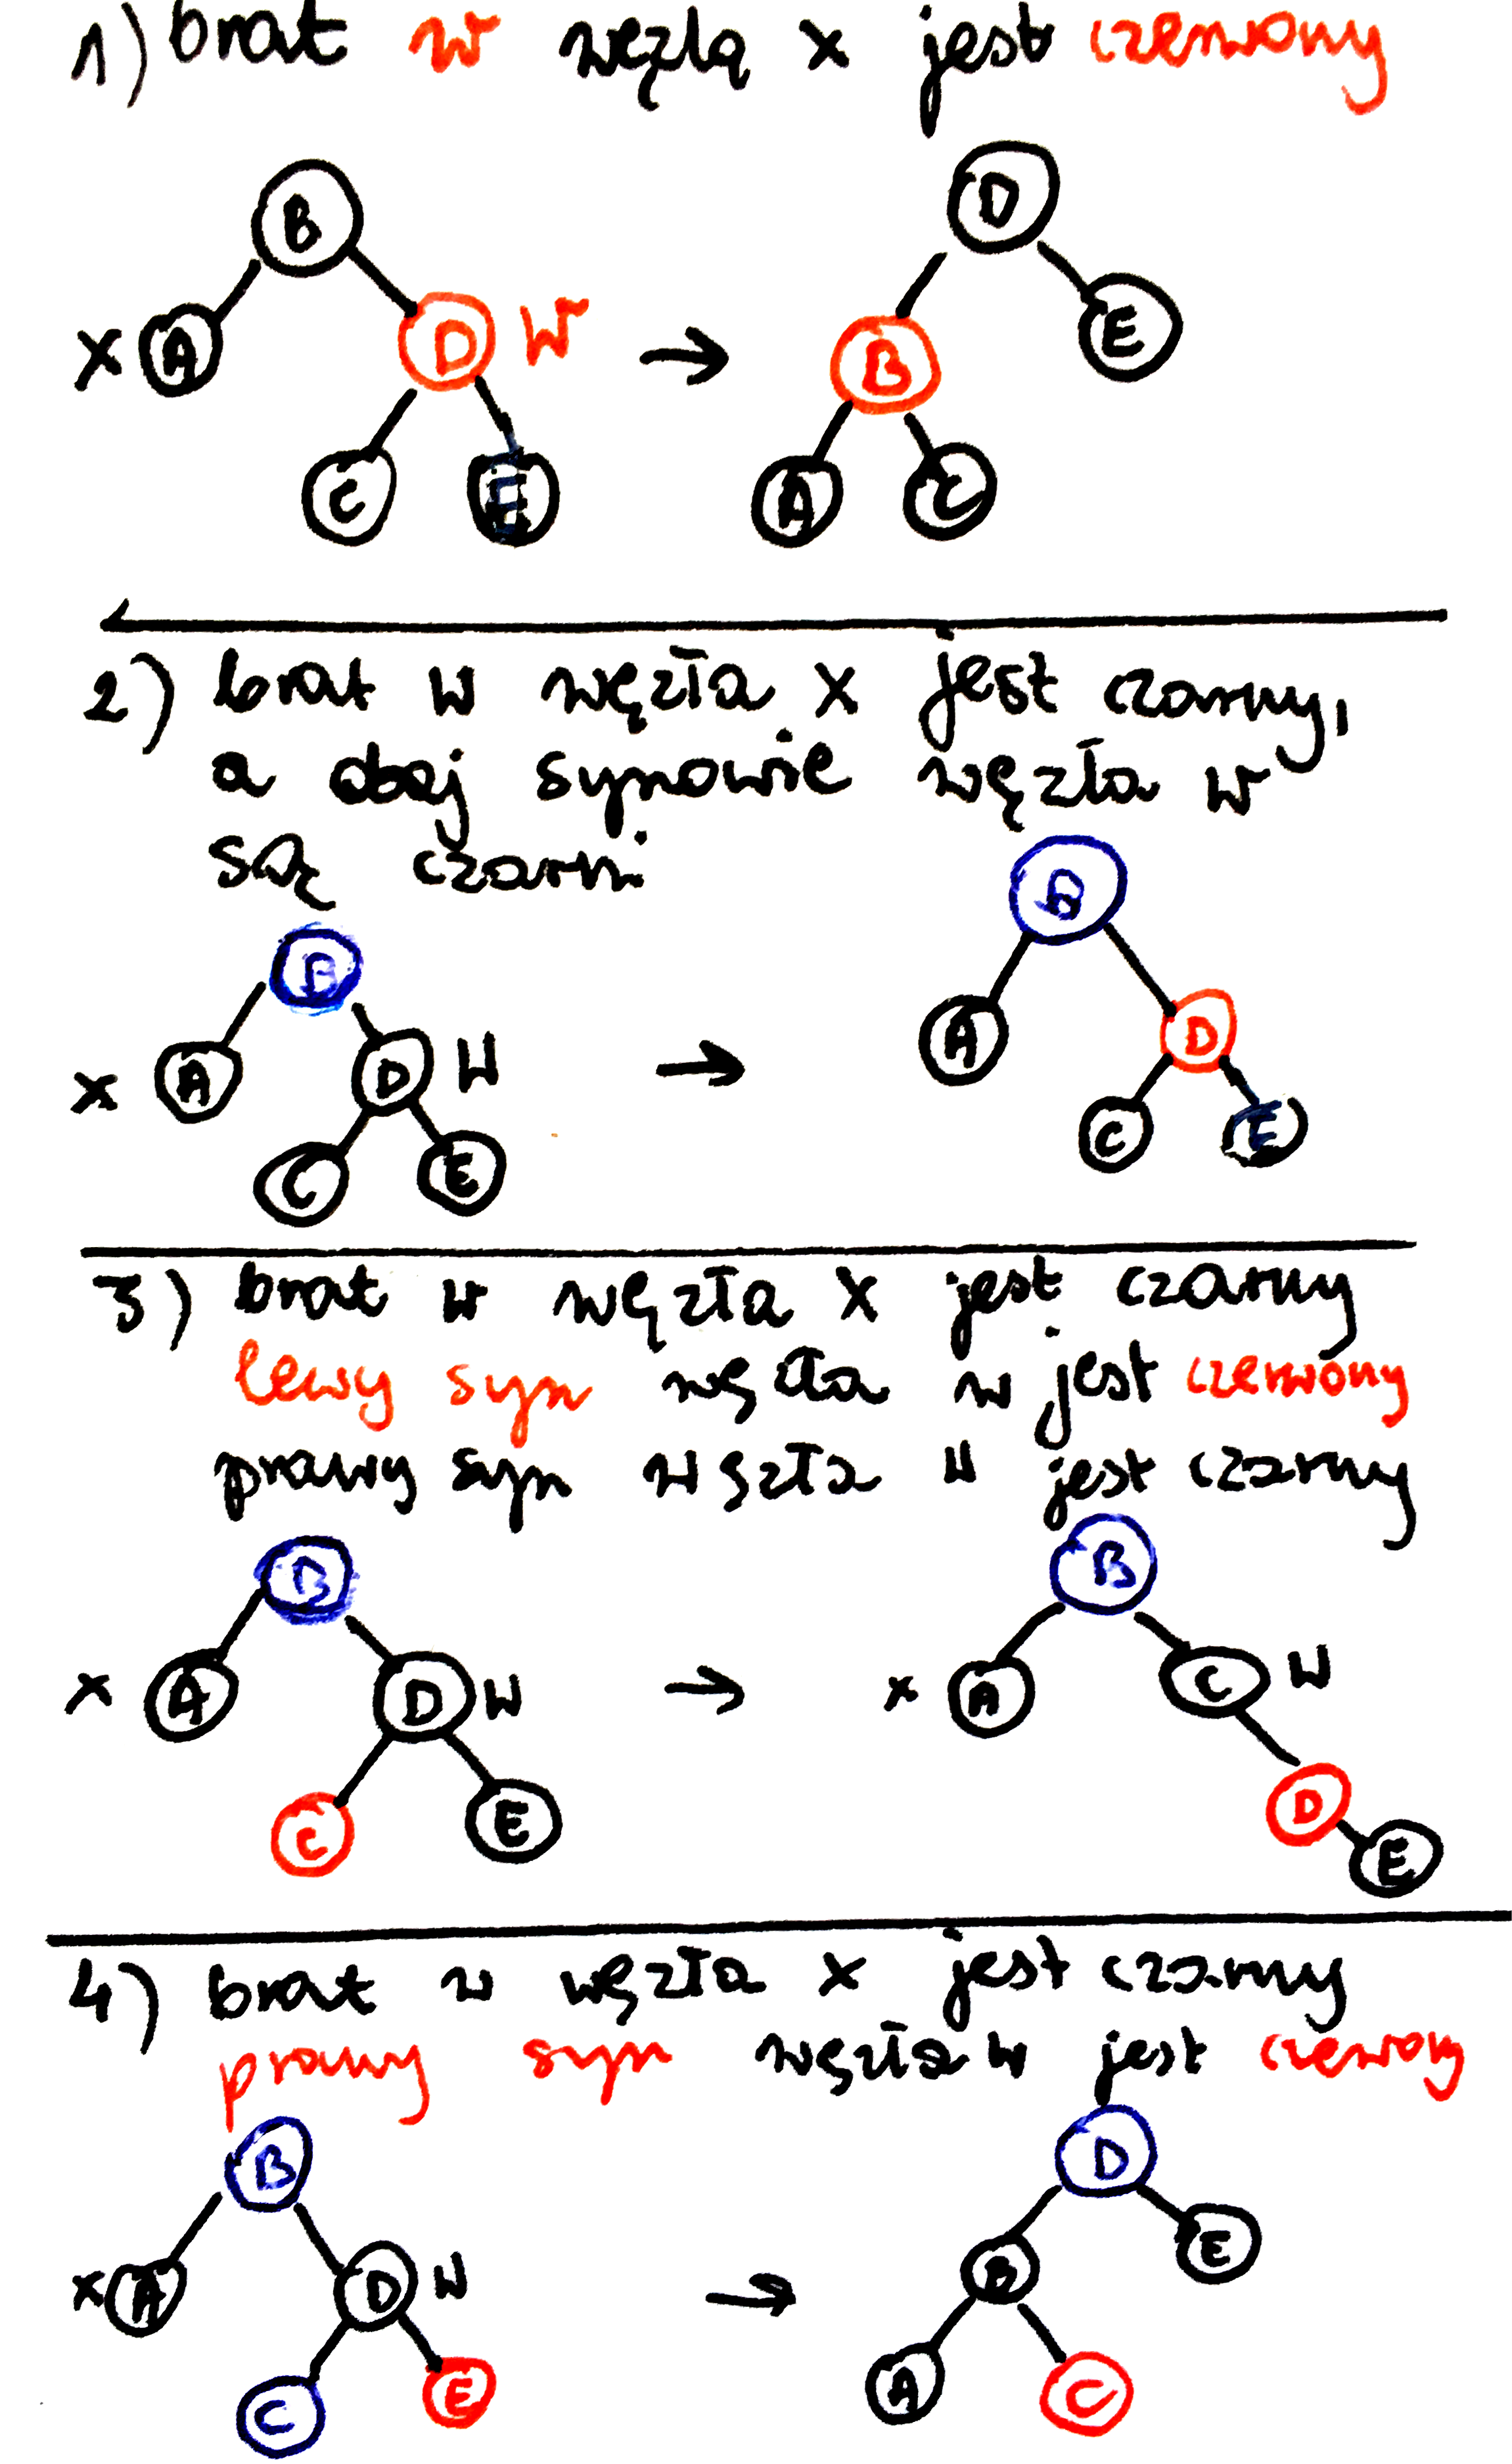
\includegraphics[width=5cm]{delete.PNG}
	 \end{figure}
	 \vspace{-0.55cm}
	WZBOGACONE STRUKTURY DANYCH: \\Dynamiczne statystyki pozycyjne \\
	\textbf{OS-SELECT}($x,i) - i$-tą statystykę pozycyjną w drzewie zawieszonym w (zwraca i-ty szukany element)$x$ $\to O(\log n)$ \\
	$k = x.left.size+1$ \\
	if $i==k$: return $x$ \\
	if $i<k$: return Os-Select($x.left,i$)\\
	else : return Os-Select($x.right, i-k$)\\	
	\textbf{OS-RANK}$(T,x)$ - którym elementem w drzewie $T$ jest $x$ (zwraca pozycję x wg inorder)  $\to O(\log n)$\\
	$r = x.left.size+1$ \\
	$y=x$ \\
	while $x \neq root$: \\
	.\quad if $y == y.parent.right$:\\
	.\quad .\quad $r = r+ y.parent.left.size+1$ \\
	.\quad $y = y.parent$ \\
	return $r$ \\
	\textbf{INTERVAL-SEARCH}($T,i$) - znajdowanie odcinka nachodzącego na $i$ z drzewa $T$ $\to O( \log n$)\\
	$\bullet$wierzchołek Interval Tree zawiera: start, end, m \\ 
	$\bullet$ m $\to$ max(x.end, x.left.m, x.right.m) \\
	$x = root(T)$ \\
	while $x \neq nil$ and ($i.start > x.end$ and $x.start>i.end$): \\
	.\quad if $x.left \neq nil$ and $i.start \leq x.left.m$: \\
	.\quad .\quad $x = x.left$ \\
	.\quad else: $x = x.right$ \\
	return $x$ \\
	\textbf{PROGRAMOWANIE DYNAMICZNE:} \\
	Problem znalezienia najkrótszej ścieżki między wierzchołkami w DAG (skierowany graf acykliczny)\\
	\textbf{NAJDŁUŻSZY ROSNĄCY PODCIĄG \\ = LIS-longest increasing subsequence} $\to O(|E|)$ \\
	\underline{Example}: $5, \underline{2}, 8,6, \underline{3}, \underline{6}, \underline{9},7$\\
	for $i=1$ to $n$: \\
	.\quad $L(j) = 1 + max \{ L(i): (i,j) \in E\}$ \\
	return $maxL(j)$ \\
	\textit{ // L(i) - długość LIS do $a_{i}$} \\
	\textbf{NAJDŁUŻSZY WSPÓLNY PODCIĄG \\ = LCS-longest common subsequence} $\to O(m*n)$ \\
	znaki nie muszą być obok siebie \\
	// wypełnienie stanów początkowych \\
	 for $i = 0$ to $n$: $C[i][0] = 0$  \\
	 for $j = 0$ to $m$: $C[0][j] = 0$\\
	 for $i = 1$ to $n$: \\
	 .\quad for $j = 1$ to $m$:\\
	 .\quad .\quad if $A[i] == B[j]$: $C[i][j] = C[i-1][j-1] + 1 $  \\
	 .\quad .\quad else : $C[i][j] = max(C[i-1][j], C[i][j-1])$ \\
	 return $C[i][j]$ \\
	 \textbf{NAJDŁUŻSZE WSPÓLNE PODSŁOWO \\ = Longest common substring $\to O(mn)$}\\
	 $\to$ największe takie $k$, dla którego istnieją indeksy $i,j$, takie że $x_{i}x_{i+1}..x_{i+k-1}=y_{j}y_{j+1}..x_{j+k-1}$ w rozwiąz. S,T-słowa\\
	 $LCSuff(S_{1..p},T_{1..q})=\{LCSuff(S_{1..p-1},T_{1..q-1})+1$ if $S_{p}=T_{q}$\\
	 $\to$ Znaleźć najdłuższy wspólny sufiks dla wszystkich par prefiksów słów. $z$- trzyma najdł. wspólne podsłowo znalezione do tej pory, $ret$ - trzyma zestaw stringów długości $z$, $i$-ostatni znak(w LCS rozmiaru$z$)\\
	 $LCSubst(S,T)=max_{1\leq j\leq n, 1 \leq j \leq n}LCSuff(S_{1..i},T_{1..j})$\\
	 $LFCSubst(S[1..m],T[1..n])$:$L= A[1..m][1..n], z=0, ret=\{\}$ for $i=1$ to $m$: for $j=1$ to $n:$\\
	 .\quad if $S[i]==S[j]$: \\
	 .\quad.\quad if $i==1$ or $j==1: L[i,j]=1$\\
	 .\quad.\quad else: $L[i,j] = L[i-1,j-1]+1$\\
	 .\quad .\quad if $L[i,j]>z$: $z=L[i,j], ret={S[i-z+1..i]}$\\
	 .\quad .\quad else if $L[i,j] = z$: $ret.add{S[i-z+1..i]}$\\
	 \textbf{EDIT DISTANCE} $\to O(m*n)$ \\
	 for $i=0$ to $m$: $E[i][0] = i$ \\
	 for $j=0$ to $n$: $E[0][j] = j$ \\
	 for $i=1$ to $m$: \\
	 .\quad for $j=1$ to $n$: \\
	 .\quad .\quad $E[i][j] = min(E[i-1][j]+1, E[i][j-1]+1, E[i-1][j-1]+\mathbb{I} _{x[i]=y[j]})$ \quad $\mathbb{I} = 0: x[i] = y[j], 1: x[i] \neq y[j]$\\
	 \textbf{KOPIEC BINARNY} \\
	 Drzewo pełne z wyłączeniem ostatniego wiersza $\to$ h: $\Theta(\log n)$ \\
	 $parent(i) = \lfloor \frac{i}{2} \rfloor$, $left(i)=2i$, $right(i)=2i+1$ \\
	 HEAPIFY($A,i$) $\to \Theta(\log n)$ naprawianie struktury kopca \\
	 BUILD HEAP($A$) $\to O(n)$ \\
	 for $i=\lfloor \frac{size(A)}{2} \rfloor$ downto $1$: Heapify($A,i$) \\
	 HEAP SORT($A,n$)$\to O(n \log n)$ \\
	 Build-Heap($A$) \\
	 for $i=1$ downto $2$: \\
	 .\quad $swap(A[1],A[i])$ \\
	 .\quad $heap.size --$ \\
	 .\quad Heapify($A,i$) \\ 
	 \textbf{KOLEJKA PRIORYTETOWA Q}\\
	 INSERT($Q,x$) $\to O(\log n)$\\
	 $Q.size++$ \\
	 $i = Q.size$ \\
	 while $i>1$ and $Q[Parent[i]] <x$: \\
	 .\quad $Q[i] = Q[Parent[i]]$ \\
	 .\quad $i = Parent[i] $ \\
	 $Q[i]=x$ \\
	 MAXIMUM($Q$) $\to O(\log n)$ \\
	 if $Q.size = 0$: return $"error"$ \\
	 Extract-Max($Q$) \\
	 if $Q.size = 0$: return $"empty queue"$ \\
	 else: \\
	 .\quad $max = Q[1]$ \\
	 .\quad $Q[1] = Q[Q.size]$ \\
	 .\quad $Q.size --$ \\
	 .\quad Heapify($Q,1$) \\
	 .\quad return $max$ \\
	 DECREASE-KEY($Q,x,new-key$): \\
	 $x.key = new-key$ \\
	 Heapify ($Q,x$) \\
	 DELETE($Q,x$)$\to O(\log n)$: \\
	 $Q[x] = Q[Q.size]$ \\
	 $Q.size--$ \\
	 Heapify($Q,x$) \\
	 \textbf{GRAFY:}\\
	 \textbf{EXPLORE}($G,v$) \\
	 $visited(v) = true$ \\
	 $previsit(v)$ \\
	 for each $(u,v) \in E$:\\
	 .\quad if not $visited(u)$: Explore($u$) \\
	 $postvisit(v)$ \\
	 \textbf{DFS - Depth First Search}($G$) $\to O(|V|+|E|)$ \\
	 for all $v \in V$: $visited(v)=false$ \\
	 for all $v \in V$: \\
	 .\quad if not $visited(v)$: Explore($G,v$) \\
	 \textbf{BFS - Breadth First Search}($G,s$) $\to O(|V|+|E|)$ \\
	 for all $v \in E$: $dist(v) = \infty $ \\
	 $dist(s) = 0$ \\
	 $Q = [s]$\\
	 while $Q$ is not empty: \\
	 .\quad $u = $Eject$(Q)$\\
	 .\quad for all $edges(u,v) \in E$: \\
	 .\quad .\quad if $dist(v) = \infty$: \\
	 .\quad .\quad .\quad Inject($Q$)$=v$ \\
	 .\quad .\quad .\quad $dist(v) = dist(u) +1$ \\
	 \textbf{DIJKSTRA}($G,s$) $\to O((|E|+|V|)\log |V|)$, kopiec binarny \\
	 for all $v \in E$: $dist(v) = \infty, \quad prev(v) = null$ \\
	 $dist(s) = 0$ \\
	 $H$ = Build-Heap($v$) \quad \textit{//dystanse jako priorytet}\\
	 while $H$ is not empty: \\
	 .\quad $u$ = Extract-Min($H$) {\color{BrickRed}$\to O(|V|)$}\\
	 .\quad for all $(u,v) \in E$: \\
	 .\quad .\quad if $dist(v) > dist(u) + l(u,v) $: \\
	 .\quad .\quad .\quad $dist(v) > dist(u) + l(u,v) $ \\
	 .\quad .\quad .\quad $prev(v) = u $\\
	 .\quad .\quad .\quad Decrease-Key($H,v$) {\color{BrickRed}$\to O(|E|)$}\\
	 \textbf{ALG BELLMANA-FORDA} $\to O(|V|*|E|)$\\
	 Gdy ścieżki mogą posiadać wagi ujemne musimy użyć mniej efektywnego, lecz bardziej wszechstronnego algorytmu Bellmana-Forda. Algorytm tworzy poprawny wynik tylko wtedy, gdy graf nie zawiera ujemnego cyklu, czyli cyklu, w którym suma wag krawędzi jest ujemna. \\
	 for all $v \in V: dist(v) = \infty, prev(v) = null$\\
	 $dist(s) = 0$ \\
	 repeat $|v|-1$ times: \\
	 .\quad for all $e \in E$: Update($e$)\\
	 UPDATE(($u,v \in E$)) \\
	 $dist(v) = min(dist(v), dist(u)+weight(u,v)$\\
	 \textbf{MINIMALNE DRZEWO ROZPINAJĄCE - MST}:\\
	 $\to$ drzewo rozpinające T, dla którego suma wag
	 $\sum_{{e}\in T}w(e)$
	 jest najmniejsza z możliwych. Dla niektórych grafów można wskazać wiele drzew rozpinających spełniających tę własność.
	 \textbf{KRUSKAL}($G$) \textit{znajduje MST}  $\to O(|E|*\lg|V|)$\\
	 for all $v \in V$: MakeSet($v$)\\
	 posortuj krawędzie $E$ wg ich wag w porządku niemalejącym\\
	 $x = []$ 
	 for all ${u,v} \in E$: \\
	 .\quad if Find($u$) $\neq$ Find($v$): {\color{BrickRed}$\to O(2*|E|)$}\\
	 .\quad .\quad $x.add(u,v)$ \\
	 .\quad .\quad Union($u,v$) {\color{BrickRed}$\to O(|V|-1)$}\\
	 MAKE-SET($x$) $\to O(|V|)$\\
	 $\pi(x) =x$ \textit{// $\pi(x) \to$ wskaźnik na ojca x} \\
	 $r(x)=0$ \textit{// $r(x) \to$ h drzewa zawieszonego w wierzchołku x}\\
	 FIND($x$) \\
	 while $x \neq \pi(x)$: $x=\pi(x)$ \\
	 return $x$ \\
	 UNION($x,y$) \\
	 $A$ = Find($x$) \\
	 $B$ = Find($y$)\\
	 if $A == B$ : return \\
	 if $r(A) > r(B)$: $\pi(B) =A$ \\
	 else: $\pi(A) = B$ \\
	 .\quad if $r(A) == r(B)$: $r(B)++$\\
	 \textbf{PRIM} \textit{znajduje MST} $\to$ złożoność jak w Dijkstrze \\
	 for all $v \in V$: $cost(v)=\infty$, \quad $prev(v)=null$ \\
	 $v_{0}$ - początkowy wierzchołek \\
	 $cost(v_{0}) =0$ \\
	 $H$ = Build-Heap($v$) \\
	 while $H$ is not empty:\\
	 .\quad $v$ = Delete-Min($H$) \\
	 .\quad for each $(v,z) \in E$:\\
	 .\quad .\quad if $cost(z) > w(v,z):$ \\
	 .\quad .\quad .\quad $cost(z) = w(v,z)$ \\
	 .\quad .\quad .\quad $prev(z) = v$ \\
	 .\quad .\quad .\quad Decrease-Key($H,z$)\\
	 \textbf{ALGORYTMY ZACHŁANNE:} \\
	 \textbf{Kodowanie Huffmana} \\
	 \underline{Example:}
	 $\bullet$ $ 44 100 \to $liczba prób na sekundę\\
	 $\bullet$ $\Gamma$  alfabet $|\Gamma|=n$ \\
	 $\bullet$ kodowanie otrzymanego ciągu $T$ \\
	 $50min\times60\times44100 \to$ liczba próbek w 50min zapisu muzyki \\
	 $\Gamma=\{A,B,C,D\}$ \\
	 $A$ $\#$powtórzeń: $70*10^6$, $B$ $\#$powtórzeń: $3*10^6$ \\
	 $C$ $\#$powtórzeń: $20*10^6$, $D$ $\#$powtórzeń: $37*10^6$ \\
	 PREFIX FREE CODE - żaden kod nie jest prefiksmem, drzewo binarne takie, że każdy węzeł jest liściem lub ma 2'óch synów. \\
	 przykładowy ciąg: AACBDC\\
	 $A\to0$, $B\to100$, $C\to101$ $D\to11$ \\
	 \vspace{-0.75cm}
	 \begin{figure}[H]
 	 	\centering
 	 	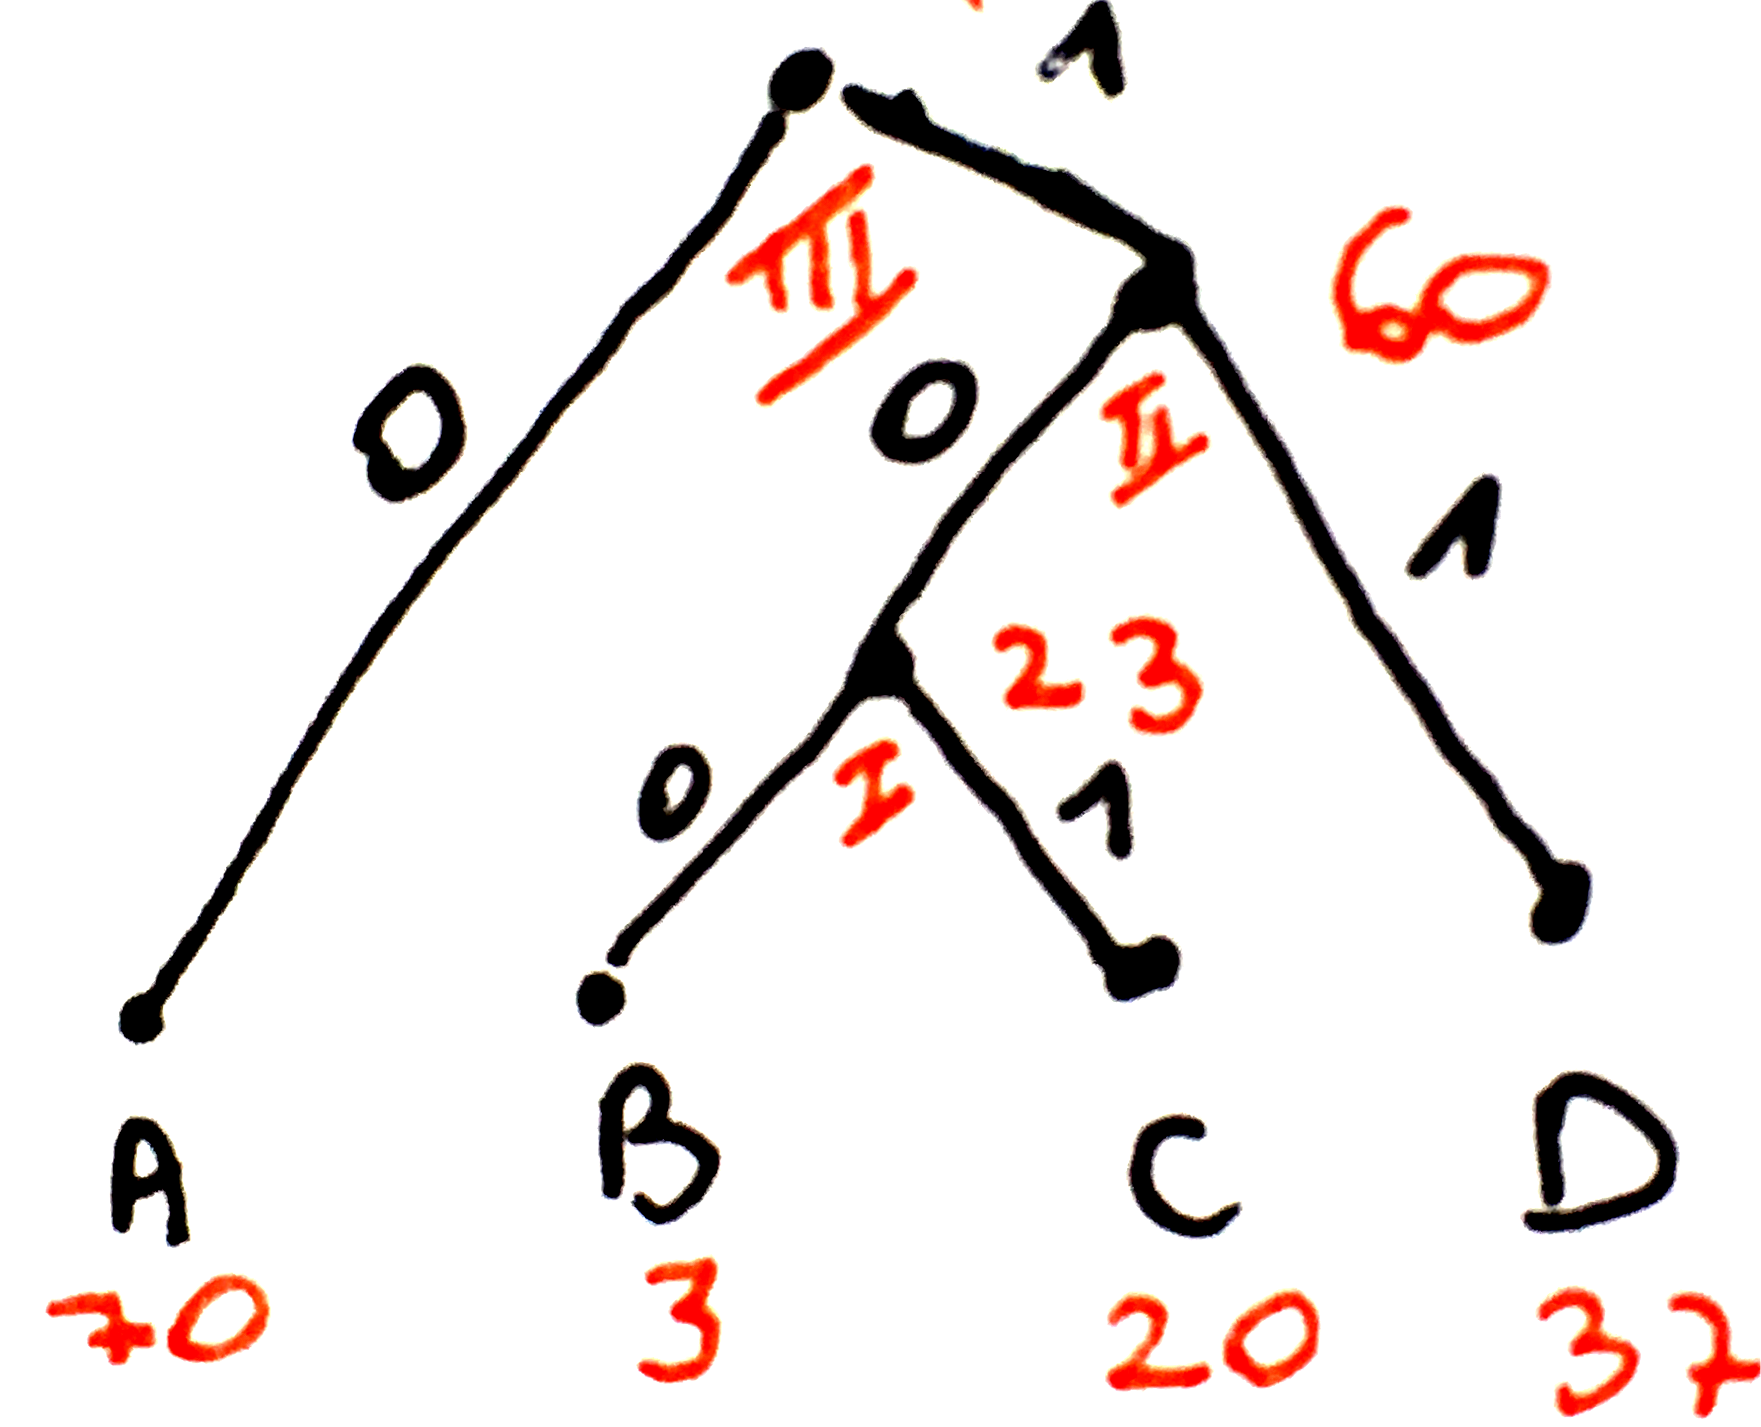
\includegraphics[width=3.5cm]{huffman.PNG}
	 \end{figure}
	 \vspace{-0.6cm}
	 koszt: $70*10^6*1 + 37*10^6*2+20*10^6*3+3*10^6*3 =$ \\ $ 213*10^6$ bitów\\
	 $f_{i} =$ liczba wystąpień symboli $i$ w ciągu $T$ \\
	 $h_{i} =$ głębokość $i$ w drzewie Huffmana\\
	 koszt: $\sum_{i=1}^{n}f_{i}h_{i}$ lub $\sum_{v \in T,v\neq root}w(v)$\\
	 HUFFMAN($T,\Gamma$) \\
	 $H$ - kolejka priorytetowa \textit{// priorytet po $f_{i}$}\\
	 for $i=1$ to $n$: Insert($H,f_{i}$)\\
	 for $k=n+1$ to $2n-1$:\\
	 .\quad i = Extract-Min($H$)\\
	 .\quad j = Extract-Min($H$)\\
	 .\quad stwórz węzeł \textit{k rodzicem, dziećmi i,j}\\
	 .\quad $f(k)=f(i)+f(j)$\\
	 .\quad insert($H,f(k)$)\\
	 \textbf{Entropia}\\
	 Który koń jest najbardziej przewidywalny? \\
	 \begin{tabular}{|c|c|c|c|}
	 	\hline 
	 	wynik/konie & A & W & P \\
	 	\hline 
	 	1 & $15\%$ & $30\%$ & $20\%$\\
	 	\hline
	 	2 & $10\%$ & $5\%$  & $30\%$ \\
	 	\hline
	 	3 & $70\%$ &$25\%$ & $30\%$ \\
	 	\hline
	 	$>$3 & $5\%$ & $40\%$ & $20\%$ \\
	 	\hline
	 \end{tabular} \\ 
	 $\%\to$ procent wygranych wyścigów \\
	 wyniki $200$ znaków \\
	 $T_{A}$ - ciąg zajmowanych miejsc przez konia $A$ \\
	 koń W: \\
	 \vspace{-0.85cm}
	 \begin{figure}[H]
 	 	\centering
 	 	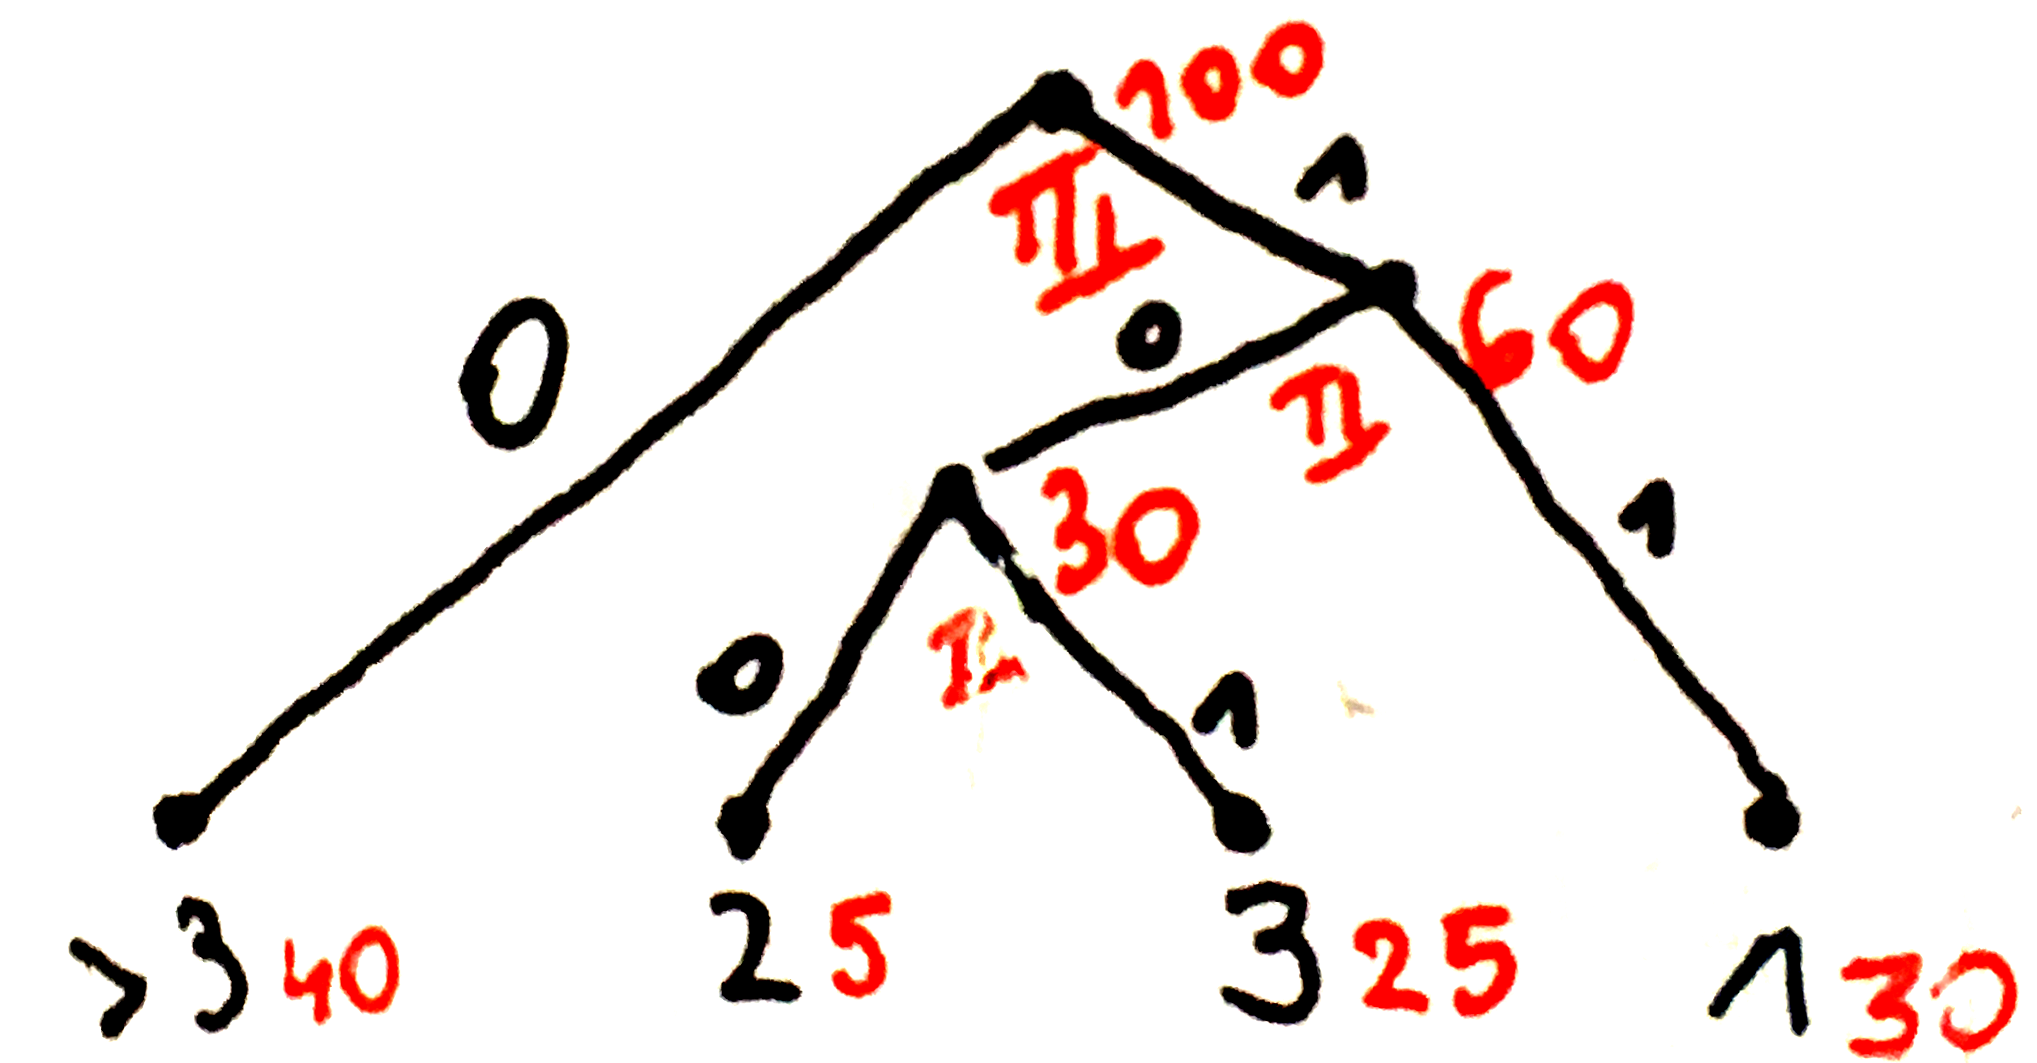
\includegraphics[width=4cm]{horse.PNG}
	 \end{figure} 
	 \vspace{-0.6cm}
	 $1\to11$, $2\to100$, $3\to101$, $>3\to0$ \\
	 $s(T_{a}) = 290$ bitów \quad $s(T_{w}) = 380$ bitów  \quad $s(T_{p}) = 400$ bitów  \\
	 $\to$ Ten koń, który najlepiej się kompresuje jest najbardziej przewidywalny. Lepiej kompresowalny $\equiv$ mniej losowo $\equiv$ bardziej przewidywalny. \\
	 Wzór na entropię:
	 $H = - \sum_{i=1}^{n}p_{i}\lg p_{i}$ \\
	 \small{
	 Programowanie dynamiczne - zadania: \\
	 \underline{zadanie} $n$ - $\#$ możliwych lokalizacji, $m_{1}..m_{n}$ - odległość lokalizacji w km od początku drogi, $p_{i}$ - oczekiwany zysk otwarcia, $k$ - $\#$km ile co najmniej powinny być od siebie oddalone restauracje. ?Alg obliczania max oczekiwanego całk. zysku?\\
	 $p_{i}=max\{ max_{j<i}{p_{j}+\alpha(m_{i},m_{j})p_{i};\quad p_{i}}$ \\
	 $\alpha(m_{i},m_{j}) = \{0$ if $ m_{i}-m_{j}<k; \quad 1$ if $ m_{i}-m_{j} \geq k$\\
	 for $i=1$ to $n: pro[i]=0$\\
	 for $i=2$ to $n$: for $j=1$ to $i-1$: \\
	 .\quad $temp=pro[j]+ \alpha(m_{i},m_{j})p_{i}$ \\
	 .\quad if $tem > p_{i}: temp=p_{i}$\\
	 .\quad if $pro[i]<p_{i}: pro[i]=p_{i}$ \\
	 \underline{zadanie} zapis złożony z $n$ znaków $s[1..n]$. Dokument tekst. utracił wszystkie odstępy. Mamy słownik $dict(w)=\{$true, jeżeli $w$ jest poprawnym słowem, false oth.; ?Alg rozstrzyga, czy z napisu $s[\bullet]$ można odtworzyć ciąg poprawnych słów.\\
	 $d[i]=\{$ true, if $s[1..i]$ jest poprawną sekwencją słów, false oth.;.\quad
	 $s[1..i]$ jest poprawną sekw. słów, wtedy gdy $s[1..j]$ ($j<i$) jest poprawną sekw. słów i $s[j+1..i]$ jest poprawnym słowem. Rekurencja: $d[i]=\{$ false if $i\leq 0$, $max_{1\leq j<i}(d[i], dict(s[j+1..i]) $ oth. \quad valid(s,n): for $i=1$ to $n$: $d[i]=false$, {\color{BrickRed}$c_{i}=0$}\\
	 .\quad for$j=1$ to $i-1$: if $d[j] \wedge dict(s[j+1..i]): d[i]=true$, {\color{BrickRed}$c_{i}=j$}.\qquad{\color{BrickRed}odtworzenie napisu: \\
	 	output(s,n,d,c):i=n, while i$>$0: print s[c[i]+1..i], i=c[i]}\\
	 \underline{zadanie}Alg obliczania długości najdłuższego podciągu palindromicznego, dla ciągu $x[1..n]$. $L(i,j)=\{L(i+1,j-1)+2,$ if $x_{i}=x_{j}$;\quad $max\{L(i+1,j),L(i,j-1)$ oth. \\
	 for $i=1$ to $n: L(i,j)=1$\\
	 for $i=1$ to $n:$ for $s=1$ to $n-i$: \\
	 .\quad $j=s+i$,$L(s,j)=cost(L,x,s,j)$,$L(j,s)=cost(L,x,j,s)$\\
	 return$L(1,n)$\\
	 cost(L,x,i,j): if $i==j$: return $L(i,j)$\\
	 else if $x_{i}==x_{j}$: \\
	 .\quad if $i+1<j-1$: return $L(i+1,j-1)+2$\\
	 .\quad else: return $2$\\
	 else: return $max(L(i+1,j),L(i,j-1))$\\
	 \underline{zadanie}$n$ wyprzedaży=$w_{1}..w_{n}\in W$, $v_{j}$-zysk wyprz.$w_{j}$, $d_{ij}$-koszt dojazdu z $w_{i}$do $w_{j}$.?Max zysk, podzbiór wyprzedaży z początkiem i końcem w domu? $C(W,j)$-zysk z najlepszej trasy, z domu kończącej się w $w_{j}$, $w_{i} \in W-\{w_{j}\}$-odwiedzony przed $w_{j}$. $C(W-\{w_{j}\},i)$- zysk do $w_{i}$ a zysk z wizyty w $w_{j}$ to $v_{j}-d{ij}$, $C(W,j)=max_{w_{i} \in W: i \neq j}\{C(W-\{w_{j}\}+v_{j}-d_{ij})$ ALG:\\ 1.inicjalizacja $C(w_{i},i)=v_{i}-d_{0j}$ dla wszystkich $1 \leq i \leq n$. 2.rozwiązywanie podproblemów zwięszając ilość $W$. 3.ostateczne rozwiązanie to $max$ z $C(W,j)-d_{j0} \to n2^{n}$ podproblemów, każdy w czasie $O(n) \to O(n^{2}2^{n})$\\
	 \underline{zadanie} dane:ciąg $n$ dodatnich liczb $a_{1}..a_{n}$i liczba $t$.?Czy pewnien pozdbiór liczb $a_{i}$ sumuje się do $t$(każda liczba raz)?\\
	 for $i=0$ to $n$: $subset[0][i]=true$\\
	 for $i=1$ to $t$: $subset[i][0]=false$\\
	 for $i=1$ to $t$: for $j=1$ to $n$: $subset[i][j]=subset[i][j-1]$\\
	 .\quad if $i\geq a[j-1]:$ $subset[i][j]=subset[i][j]$ or\\ $subset[i-a[j-1]][j-1]$ \\
	 .\quad.\quad return $subset[t][n]$\\
	 $subset[i][j]==true$ jeżeli jest podzbiór $a[0..j-1]$, którego suma jest równa $i$.\\
	 \underline{zadanie}Monety. Czy można uzbierać kwotę $V$, używając monet o nominałach $x_{1}..x_{n}.$? $A[v]$-predykat, który ocenia czy da się uzbierać dla $v$. $A[v]=OR_{1 \leq i \leq n}\{A(v-x_{i})$ if $x_{i}<v$; $false$ oth.; Alg: $A[0]=true$\\
	 for $i=1$ to $V$: $A[i]=false$\\
	 for $v=1$ to $V$: for $j=1$ to $n$: if $x_{j} \leq v$: $A[v]=A[v]vA[v-x_{j}]$\\
	 .\quad else: $A[v]=false$\\
	 return $A[v] \to O(nV)$ \qquad ?każdy nominał tylko raz:\\
	 $A(n,V)=A(n-1,V-x_{n})$ or $A(n-1,V)$\\
	 $A(i,V)=true \to$ jeśli się da dla $x_{1}..x_{i}$ \\
	 for $i=1$ to $n$: for $j=v-1$ dto $0$: if $A[j]==true$:$A[j+x_{i}]=true$
	 ?max $k$ monet: if $k>1$: $A(k,v)=max_{x_{i}<v}A(k-1,v-x_{i})$\\
	 else: $A(k,v)=(x_{1}..v)$or$(x_{2}==v)..(x_{n}==v)$\\
	 $A(k,v)==true$ to da się $\to O(nKV)$ tablica K$\times$V, n- możliwość rekurencji początkowej\\
	 \underline{zadanie}?Dla danych $m$ miejsc podziału w słowe dł. $n$, podaj alg. który znajduje minimalny koszt podzielenie tego słowa na $m+1$ części.? Np podział na pozycji $3$ $20-to$ literowego słowa uzyskamy łączny koszt: $20+17=37$.;\quad Odp. $i,j \gets$ miejsca z $m$ ($i \leq j$)\\ wskaż minimialny koszt obcinając podciąg zaczynjący się od $i$, kończący się w $j$ (włącznie) $\to cost(i,j)$ Rekursja: 1.przeglądnie wszystkich znaczników $k$, takoch, że $i<k<j$ 2.potem z tych punktów wybieramy jeden, taki że $(j-1)+cost(i,k+1)+cost(k+i,j)$ jest najmniejsze 3.$j-i$ jest długością tego podciągu i dodajemy do tego min cost podziału na mniejsze podciągi 4.best case: $i=j \to$ return $0$; $\to O(m^{2})$ spamiętanie dla każdej pary $(i,j)$ + $O(m)$ liczba pozycji w tablicy i porównywanie $\to O(m^3)$\\
	 
	 }
	 
	 
\end{multicols*}
\end{document}